\section{Study3: Quantify the impact of uplift events}
To quantify the restoring impact of uplift event,
in this section, we propose to model the impact as the teen's behavioral differences in two cases:
1) stressful intervals unaffected by uplift events (SI), and 2) stressful intervals impacted by uplift events (U-SI).
Multiple stress and positive emotion related measures are proposed to describe the correlation between SI and U-SI,
and we quantify such differences as correlations using a two-sample based statistical method.

\subsection{Restoring Patterns and Behavioral Measures}
\label{subsec:pattern}
To extract the restoring patterns \bm{${A}$} for each type of uplift events,
we describe a teen's positive and stressful behavioral measures in SI and U-SI sets from three aspects:
posting behavior, stress intensity, and linguistic expressions.
%For an uplift event $u$ with type $U^{'}$,
%a stressor event $e$ with type $S^{'}$,
%let $F$:$(u, U^{'}, e, S^{'}) \rightarrow $ \bm{${A}$}
%(\bm{${A}$} is a multidimensional vector) be the stress-buffering effect of uplift event $u$
%conducted on the stress caused by stressor event $e$.

\textbf{Posting behavior}.
Stress could lead to a teen's abnormal posting behaviors,
reflecting the teen's changes in social engagement activity.
For each stressful interval,
we consider three measures of posting behaviors in each time unit (day),
and present each measure as a corresponding series.
The first measure is \emph{posting frequency},
representing the total number of posts per day.
Research in \cite{Li2017Analyzing} indicates that overwhelmed teens usually tend to post more to express their stress for releasing
and seeking comfort from friends.
Further, the second measure \emph{stressful posting frequency} per day
is based on previous stress detection result and highlights the stressful posts among all posts.
Similarly, the third measure is the \emph{positive posting frequency}, indicating the number of positive posts per day.
The forth measure \emph{original frequency} is the number of original posts, which filters out re-tweet and shared posts.
Compared to forwarded posts, original posts indicate higher probability that teens are talking about themselves.
Thus for each day in current interval, the teen's posting behavior is represented as a four-dimension vector.

\textbf{Stress intensity}.
We describe the global stress intensity during a stressful interval through four measures:
\emph{sequential stress level, length, RMS,} and \emph{peak}.
Basically, \emph{stress level} per day constructs a sequential measure during a stressful interval,
recording stress values and fluctuation on each time point.
The \emph{length} measures the lasting time of current stressful interval.
As uplift events might conduct impact on overwhelmed teens,
and postpone the beginning or promote the end of the stressful interval,
we take the \emph{length} as a factor representing the interval stress intensity.
To quantify the intensity of fluctuations for stress values,
we adopt the \emph{RMS} (root mean square) of stress values through the interval as the third measure.
In addition, the \emph{peak} stress value is also a measure to show the maximal stress value in current interval.

\textbf{Linguistic expressions}.
We extract the teen's positive and stressful expressions from the content of posts in SI and U-SI sets, respectively.
The first linguistic measure is the frequency of \emph{positive word},
which represents the positive emotion in current interval.
The second measure is the frequency of \emph{uplift event topic words} in six dimensions,
reflecting the existence of uplift events.
Another important factor is wether existing \emph{self-mentioned words} (i.e., \emph{'I','we','my'}).
Self-mentioned words show high probability that the current stressor event and stressful emotion is related to the author,
rather than the opinion about a public event or life events about others.

Except uplift-related linguistic descriptions, we also take stressful linguistic characters as measures,
which is opposite with positive measures, while also offers information from the complementary perspective.
The first stressful linguistic measure is the frequency of \emph{stressor event topic words} in five dimensions,
which represents how many times the teen mentioned a stressor event,
indicating the degree of attention for each type of stressor event.
The frequency of \emph{pressure words} is the second stressful linguistic measure,
reflecting the degree of general stress emotion during the interval.
We adopt this measure specifically because in some cases teens post very short tweets with only stressful emotional words,
where topic-related words are omitted.

Next,
based on the posting behavior, stress intensity and linguistic measures from both the stressful and positive views,
we quantify the difference between SI and U-SI sets, thus to measure the impact of uplift events.

\subsection{Quantify the Correlation}
In our problem,
there are two sets of stressful intervals to compare:
the SI set and the U-SI set,
containing stressful intervals unaffected by uplift events
and stressful intervals impacted by uplift events, respectively.
The basic elements in each set are stressful intervals,
i.e., the sequential stress values in time line,
which are modeled as multi-dimensional points according to the three groups of measures in section \ref{subsec:pattern}.
Thus we formulate this comparison problem as finding the correlation between the two sets of multi-dimension points.
Specifically, we adopt the multivariate two-sample hypothesis testing method
\cite{Li2017Correlating,Johnson2012Applied} to model such correlation.
In this two-sample hypothesis test problem,
the basic idea is judging whether the multi-dimension points (i.e., stressful intervals)
in set SI and set U-SI are under different statistical distribution.
Assuming the data points in SI and U-SI are randomly sampled from distribution $F^{(1)}$ and $F^{(2)}$, respectively,
then the hypothesis is denoted as:
\begin{equation}
H_0: F^{(1)} =F^{(2)} \quad versus \quad H_1: F^{(1)} \neq F^{(2)}.
\end{equation}

Under such hypothesis,
$H_0$ indicates points in SI and U-SI are under similar distribution,
while $H_1$ means points in SI and U-SI are under statistically different distributions,
namely uplift events have conducted obvious restoring impact on current stressed teen.
Next, we handle this two-sample hypothesis test problem based on both positive and stressful behavioral measures
(i.e., \emph{posting behavior}, \emph{stress intensity} and \emph{linguisitc expressions}),
thus to quantify the restoring patterns of uplift events from multi perspectives.

As a classic statistical topic, various algorithms have been proposed to solve the two-sample hypothesis testing problem.
Since each point in the two sets (SI and U-SI) is depicted in multi-dimensions,
here we take the KNN (k nearest neighbors) \cite{Schilling1986Multivariate}
based method to judge the existence of significant difference between SI and U-SI.
For simplify, we use the symbol $A_1$ to represent set SI,
and $A_2$ represent set U-SI,
namely $A_1$ and $A_2$ are two sets composed of stressful intervals.
In the KNN algorithm,
for each point $\ell_{x}$ in the two sets $A_1$ and $A_2$,
we expect its nearest neighbors (\emph{the most similar points}) belonging to the same set of $\ell_x$,
which indicates the difference between the points in the two cases.
The model derivation process is described in detail in the \ref{mod:mod1} part of the appendix.

\subsection{Temporal Order}
\label{sec:temporal}
To measure the temporal order of stress changes in the two sets of intervals (SI and U-SI) ,
we further compare each interval with the front and rear adjacent intervals, respectively.
%denoted as $SI^{front}$, $SI^{rear}$, $USI^{front}$, $USI^{rear}$.
%We compare the intensity of stress changes in four situations,
%
%where $g(.)$ is the function comparing two sets:
%1) $g(SI,SI^{front}$) returns if intensive change happens when stressful intervals begin;
%2) $g(SI,SI^{rear}$) returns if the teen's stress change intensively after the stressful intervals end
%3) $g(USI,USI^{front}$) returns if intensive change happens when stressful intervals affected by uplift events appears.
%4)  $g(USI,USI^{rear}$) returns if stress change intensively after stressful intervals affected by uplift events end.
%
%%\\\vspace{1mm}
%%\textcircled{1} $g(SI,SI^{front}$) returns if intensive change happens when stressful intervals begin.
%%\\\vspace{1mm}
%%\textcircled{2} $g(SI,SI^{rear}$) returns if the teen's stress change intensively after the stressful intervals end.
%%\\\vspace{1mm}
%%\textcircled{3} $g(USI,USI^{front}$) returns if intensive change happens when stressful intervals affected by uplift events appears.
%%\\\vspace{1mm}
%%\textcircled{4} $g(USI,USI^{rear}$) returns if stress change intensively after stressful intervals affected by uplift events end.
%%%�������ͼ��
Here we adopt the t-test method as the intensity computation function,
to observe whether the occurrence of uplift events relieve the monotonic negative effect and the monotonic positive effect.
Details are presents in part \ref{mod:mod2} of the appendix.

The overall pipeline for identifying the restoring impact of uplift events is presented in algorithm \ref{alg:alg4}

%\subsection{Overall Algorithm}
%The overall pipeline for identifying the restoring impact of uplift events is presented in algorithm \ref{alg:alg4}.
%1) To quantify the restoring impact of uplift events,
%we first extract uplift events and stressful intervals from the teen's microblogs.
%All stressful intervals are classified into two sets:
%the set of stressful intervals affected by uplift events (SI),
%and the set of stressful intervals impacted by uplift events (U-SI).
%2) To judge if SI are statistically different with U-SI,
%next, the two-sample hypothesis testing method is conducted on the two sets
%with multi positive and stressful measures (posting behavior, stress intensity and linguistic expressions).
%3) To further judge the monotonous restoring intensity of each type of uplift events,
%the final step comes to comparing SI and U-SI with adjacent intervals, respect to temporal order.

\subsection{Results}
\paragraph{Set up}
We adopt the commonly used Pearson correlation algorithms to compare with the two sample statistical method in this study.
As a widely adopted measure of the linear correlation between two variables,
the Pearson correlation method computes a value in the range ($-1,1$),
where 1 denotes total positive linear correlation,
0 denotes no linear correlation,
and $-1$ is total negative linear correlation.
In our two sample statistical procedure,
to calculate the distance between two $n$ dimension points $X$ and $Y$,
we adopt the Euclidean metric.

\begin{table}
\begin{center}
\caption{\small{Quantify the impact of scheduled uplift school events using KTS and baseline method.}}
\small{
\begin{tabular}{l c c c c c} \\ \hline \hline
&	\emph{Practical}	&	         	&	\emph{New year}	&	\emph{Sports}	&	\emph{}	\\
&	\emph{activity}	&	\emph{Holiday}	&	\emph{party}	&	\emph{meeting}	&	\emph{All}	\\ \hline
Size of U-SI	&	219 	&	339 	&	235 	&	226 	&	1,019 	\\
Pearson         &54.52\%	&	78.39\%	&	63.39\%	&	58.74\%	&	69.52\% \\
KTS$^1$             &55.65\%	&	70.97\%	&	56.45\%	&	54.84\%	&	65.32\% \\
\hline \hline
\end{tabular}
\begin{tablenotes}
\footnotesize
\item[1] $^1$KTS denotes the knn-based two sample method adopted in this research.
\end{tablenotes}
}
\label{tab:schedule}
\end{center}
\end{table}

\begin{table*}
\begin{center}
\caption{\small{Monotonous stress intensity changes in U-SI and SI intervals compared with adjacent intervals.}}
%\resizebox{\textwidth}{15mm}{
\small{
\begin{tabular}{l cccccc cccccc} \\\hline\hline
\multirow{2}{1cm}{}
&\multicolumn{2}{c}{School life}
&\multicolumn{2}{c}{Romantic}
&\multicolumn{2}{c}{Peer relationship}
&\multicolumn{2}{c}{Self-cognition}
&\multicolumn{2}{c}{Family life}
&\multicolumn{2}{c}{All types}\\
&U-SI	    &	SI	        &U-SI	    &SI	        &U-SI	   &SI	
&U-SI	    &	SI	        &	U-SI	&SI	        &U-SI	   &SI\\  \hline
\# Interval         &   365	        &	514	        &	536	        &	587	        &128	    &	391	        &	564	           &	609	            &	321	        &	481	        &	1,914	    &2,582	 \\
Front $\rightarrow$ I &	0.7260 	&	0.7879 	&	0.6903 	&	0.7751 	&	0.7422 	&	0.8159 	&	0.7004 	&	0.7767 	&	0.6791 &	0.7796 	&	0.7017 	&   0.7851\\
I $\rightarrow$ rear  &	0.7589 	&	0.7840 	&	0.7463 	&	0.7905 	&	0.7813 	&	0.8261 	&	0.7500 	&	0.7915 	&	0.7414 	&	0.7942 	&	0.7513 	&   0.7955\\ \hline \hline
\end{tabular}}%}}
\label{tab:fontrear}
\end{center}
\end{table*}

\paragraph{Restoring Impact of scheduled uplift events}
Basically, we focused on four kinds of scheduled positive events:
\emph{practical activity}, \emph{holiday}, \emph{new year party} and \emph{sports meeting}.
For each of the four scheduled positive events,
we quantify the restoring impact and temporal order
based on corresponding SI and U-SI interval sets of the 124 students.
Table \ref{tab:schedule} shows the experimental results,
where 54.52\%, 78.39\%, 63.39\%, 58.74\% significant restoring impact are detected for the four specific scheduled positive events, respectively, with the total accuracy to 69.52\%.

For comparison,
our knn-based two sample method (denoted as \emph{KTS}) outperforms the baseline method
with the best improvement in \emph{new year party} to 10.94\%,
and total improvement to 6\%.
The correlation of uplift events for \emph{linguistic expression},
\emph{stress intensity} and \emph{post behaviors} towards five types of stressor events
are shown in Figure \ref{fig:correlation},
among which the uplift events conduct most intensive restoring impact in 'school life' and 'peer relationship' dimensions.

\begin{figure}[H]
\centering
\caption{Correlation towards each types of stressor events}
\includegraphics[width=\linewidth]{figs/correlation2.eps}%figs/correlation.eps
\label{fig:correlation}
\end{figure}




\paragraph{Monotonous stress changes caused by uplift events}
Further more,
to verify the monotonous stress changes when an uplift event impacts a stressful interval,
we collected 1,914 stressful intervals in U-SI,
and 2,582 stressful intervals impacted by uplift events in SI.
For each stressful interval in SI and U-SI,
we quantify its stress intensity by comparing with the front and rear adjacent intervals, respectively.
Here four situations are considered and compared according to the temporal order in Section \ref{sec:temporal},
as shown in Table \ref{tab:fontrear},
where the \emph{ratio of intervals} detected with monotonous increase from the \emph{front interval} to \emph{stressful interval} (denoted as \emph{front$ \rightarrow$ I}),
and monotonous decrease from the \emph{stressful interval} to the \emph{rear interval} (denoted as \emph{I $\rightarrow$ rear}) are listed.
Under the impact of uplift events,
both the ratio of intensive stress increase in \emph{front$ \rightarrow$ I}
and the ratio of intensive stress decrease in \emph{I $\rightarrow$ rear} are decreased,
showing the effectiveness of the two sample method for quantifying the impact of uplift events,
and the rationality of the assumption that uplift events could help ease stress of overwhelmed teens.

\paragraph{Integrating the stress-buffering effect into stress prediciton}
Further, to measure the effectiveness of our method for quantifying the restoring impact of uplift events,
we integrate the impact of uplift events into traditional stress series prediction problem,
and verify whether the restoring pattern of uplift events could help improve the prediction performance.
Here we choose the SVARIMA (Seasonal Autoregressive Integrated Moving Average) algorithm \cite{Shumway2006Time},
which is proved to be suitable for teens' linear stress prediction problem \cite{Li2015Predicting},
due to the seasonality and non-stationarity of teens' stress series.
The basic stress prediction is conducted using SVARIMA approach,
in the set of stressful intervals impacted by uplift events (U-SI).
Since stressor events cause the fluctuation of stress series from normal states,
%and the simple series prediction method is difficult to handle such exception.
to eliminate the interference,
we simply consider the prediction problem in those stressful intervals rather than randomly picked out stress series.
The impact of uplift events are utilized as adjust values to modify the stress prediction result.
Four metrics are adopted to measure the stress forecasting problem,
where \emph{MSE}, \emph{RMSE} and \emph{MAD} measure absolute errors and \emph{MAPE} measures relative errors.
%For all real stress value $\overline{s_i}$ and predicted stress value $s_i$ in predicting sequence $<s_1,\cdots,s_n>$,
%$MSE = \frac{1}{n}\sum_{i\in[1,n]}(s_i-\overline{s_i})^2$,
%$RMSE = \frac{1}{n}\sqrt{\sum_{i\in[1,n]}(s_i-\overline{s_i})^2}$,
%$MAD = \frac{1}{n}\sum_{i\in[1,n]}|s_i-\overline{s_i}|$,
%and $MAPE = \frac{1}{n}\sum_{i\in[1,n]}{|s_i-\overline{s_i}|/s_i}$.

\begin{table*}
\caption{Compare the stress forecast performance under three restoring patterns of uplift events.}
\begin{minipage}{\linewidth}
\centering
\resizebox{\textwidth}{20mm}{
\begin{tabular}{l cccc cccc cccc cccc} \\\hline\hline%\toprule
\multirow{2}{1cm}{}&\multicolumn{4}{c}{None}
    &\multicolumn{4}{c }{Uplift (L)}
    &\multicolumn{4}{c }{Uplift (S)}
    &\multicolumn{4}{c}{Uplift (P)}\\
    &\scriptsize{MSE} &\scriptsize{RMSE} &\scriptsize{MAPE} &\scriptsize{MAD}
    &\scriptsize{MSE} &\scriptsize{RMSE} &\scriptsize{MAPE} &\scriptsize{MAD}
    &\scriptsize{MSE} &\scriptsize{RMSE} &\scriptsize{MAPE} &\scriptsize{MAD}
    &\scriptsize{MSE} &\scriptsize{RMSE} &\scriptsize{MAPE} &\scriptsize{MAD} \\\midrule					
School life
&   0.0856 	&	0.2926 	&	0.4852 	&	0.1146	&	0.0259 	&	0.1609 	&	0.2991 	&	0.0923 	
&	0.0297 	&	0.1723 	&	0.3135 	&	0.0899 	&	0.0223 	&	0.1493 	&	0.3438 	&	0.0931 	\\
Romantic
&   0.0703 	&	0.2651 	&	0.3555 	&	0.1083 	&	0.0291 	&	0.1706 	&	0.2832 	&	0.0919 	
&	0.0379 	&	0.1947 	&	0.2941 	&	0.1026 	&	0.0332 	&	0.0835 	&	0.2746 	&	0.1240 	\\
Peer relationship
&   0.2800 	&	0.5292 	&	0.3256 	&	0.1697 	&	0.3140 	&	0.5604 	&	0.3626 	&	0.1202 	
&	0.2972 	&	0.5452 	&	0.3060 	&	0.1298 	&	0.2557 	&	0.1472 	&	0.3481 	&	0.1458 	\\
Self-cognition
&   0.0445 	&	0.2110 	&	0.3066 	&	0.1895 	&	0.0345 	&	0.1857 	&	0.2721 	&	0.1653 	
&	0.0366 	&	0.1913 	&	0.2557 	&	0.0754 	&	0.0245 	&	0.0862 	&	0.2863 	&	0.1447 	\\
Family life
&   0.1602 	&	0.4002 	&	0.3291 	&	0.1587 	&	0.0889 	&	0.2982 	&	0.2891 	&	0.0944 	
&	0.0378 	&	0.1944 	&	0.2952 	&	0.0842 	&	0.1827 	&	0.0979 	&	0.3148 	&	0.1131 	\\
All	
&   0.1281 	&	0.3579 	&	0.3604 	&	0.1482	&	0.0985 	&	0.3138 	&	0.3012 	&	0.1128 	
&	0.0878 	&	0.2964 	&	0.2929 	&	0.0964 	&	0.1037 	&	0.1128 	&	0.3135 	&	0.1241 	\\ \hline\hline
\end{tabular}}
\end{minipage}\\
\begin{minipage}{\linewidth}
\centering
\resizebox{\textwidth}{20mm}{
\begin{tabular}{l cccc cccc cccc cccc} \\\hline\hline%\toprule
\multirow{2}{1cm}{}&\multicolumn{4}{c}{Uplift (L\&S)}
    &\multicolumn{4}{c }{Uplift (L\&P)}
    &\multicolumn{4}{c }{Uplift (S\&P)}
    &\multicolumn{4}{c}{Uplift (L\&S\&P)}\\
    &\scriptsize{MSE} &\scriptsize{RMSE} &\scriptsize{MAPE} &\scriptsize{MAD}
    &\scriptsize{MSE} &\scriptsize{RMSE} &\scriptsize{MAPE} &\scriptsize{MAD}
    &\scriptsize{MSE} &\scriptsize{RMSE} &\scriptsize{MAPE} &\scriptsize{MAD}
    &\scriptsize{MSE} &\scriptsize{RMSE} &\scriptsize{MAPE} &\scriptsize{MAD} \\\midrule					
School life
&	0.0283 	&	0.1682 	&	0.2934 	&	0.0824 	&	0.0261 	&	0.1616 	&	0.2770 	&	0.0768 	
&	0.0342 	&	0.1849 	&	0.2629 	&	0.0590 	&	0.0132 	&	0.1149 	&	0.2364 	&	0.0717 	\\
Romantic
&	0.0219 	&	0.1480 	&	0.2532 	&	0.0839 	&	0.0180 	&	0.1342 	&	0.2644 	&	0.0952 	
&	0.0176 	&	0.1327 	&	0.2549 	&	0.0823 	&	0.0251 	&	0.1584 	&	0.2507 	&	0.0891 	\\
Peer relationship
&	0.2361 	&	0.4859 	&	0.3182 	&	0.1300 	&	0.2349 	&	0.4847 	&	0.3283 	&	0.1189 	
&	0.2351 	&	0.4849 	&	0.3558 	&	0.1297 	&	0.2341 	&	0.4838 	&	0.3096 	&	0.1093 	\\
Self-cognition
&	0.0329 	&	0.1814 	&	0.2942 	&	0.0946 	&	0.0262 	&	0.1619 	&	0.2791 	&	0.0858 	
&	0.0245 	&	0.1565 	&	0.2740 	&	0.0945 	&	0.0144 	&	0.1200 	&	0.2580 	&	0.0739 	\\
Family life
&	0.1489 	&	0.3859 	&	0.2750 	&	0.1244 	&	0.0395 	&	0.1987 	&	0.2853 	&	0.0939 	
&	0.0484 	&	0.2200 	&	0.2946 	&	0.0992 	&	0.0378 	&	0.1944 	&	0.2645 	&	0.0848 	\\
All
&	0.0936 	&	0.3060 	&	0.2868 	&	0.1031 	&	0.0689 	&	0.2626 	&	0.2868 	&	0.0941 	&	0.0720 	&	0.2683 	&	0.2884 	&	0.0929 	&	0.0649 	&	0.2548 	&	0.2638 	&	0.0858 	\\ \hline\hline
\end{tabular}}
\begin{tablenotes}
        \footnotesize
        \item[1] $^1$ Three restoring pattern measures: 'L' represents \emph{linguistic expression}, 'S' represents \emph{stress intensity}, and 'P' represents \emph{posting behavior}.
      \end{tablenotes}
\end{minipage}
\label{tab:forecast}
\end{table*}

We integrate the impact of uplift events into stress prediction.
The experimental set contains 1,914 stressful intervals under the impact of uplift events (U-SI).
%The number of each type of uplift events and stressful intervals are lists in Table \ref{tab:fontrear}.
As shown in Table \ref{tab:forecast},
the original prediction result using only SVARIMA method
achieves 0.1281 MSE, 0.3579 RMSE, 0.3604 MAPE and 0.1482 MAD ($L = 7$, $\alpha = 0.5$).
Then we integrate the impact of each type of uplift events into stress prediction.
Specifically, for uplifts with obvious restoring impact (under the L\&S\&P pattern),
the average stress level during historical restoring intervals are integrated to modify the result,
with adjusting the parameter $\alpha$ (details see \ref{sec:parameter}).
After the modification,
the prediction performance achieves 0.0649 MSE,	0.2548 RMSE, 0.2638 MAPE and 0.0858 MAD,
reducing the prediction errors efficiently (with MSE, RMSE, MAPE and MAD reduced by 49.34\%, 28.81\%, 26.80\% and 42.11\%, respectively).


\begin{figure*}
\centering
\caption{Teens' stress forecast performance under different lengths of predicting windows.}
\includegraphics[width=\linewidth]{figs/predictWindow2.eps}
\label{fig:length}
\end{figure*}

Further,
we present the prediction result under the impact of uplift events under different lengths of prediction windows,
ranging from 1 to 10 days, as shown in \ref{fig:length}.
With the window length increasing,
the prediction error shows decreasing trend in all metrics.
The reason is that longer prediction window takes more previous predicted results,
and the error accumulates with more predicted values taken into the next step prediction.
Among the five dimensions of events,
the prediction for school life stress achieves the best performance.
On one side,
more uplift events and stressors about school life events are detected from teens microblogs,
providing sufficient data in prediction.
On the other side,
stress coming from school life is the most common stress in the student group,
with relative stable periodicity and high frequency.


\paragraph{Contribution of each restoring measure}
We conduct experiments with different restoring patterns included respectively to show
its contribution to the impact of uplift events during prediction.
Four groups of situations are considered here, as shown in Table \ref{tab:forecast},
considering
1) all the stress intensity, linguistic expression and post behavior measures (the L\&S\&P pattern),
2) any two of the three measures included (the L$|$S, L\&P, and S\&P patterns),
3) only one of the three measures included (the L, S, or P patterns),
and 4) none measure included.
We integrate the impact of uplift events under the four situations into stress prediction
using the parameter $\alpha$,
as overlapping $\alpha \times S_{historical}$,
where $S_{historical}$ is the average stress level in historical restoring intervals.
The detailed adjust process of $\alpha$  is presenting in section \ref{sec:parameter}.
Here we present the prediction result when $\alpha = 0.5$ in each dimension of stress respectively.
Results show that the correlation in the L\&S\&P pattern outperforms other patterns
(0.0649 MSE, 0.2548 RMSE, 0.2638 MAPE and 0.0858 MAD),
showing the effectiveness of considering all the three correlations.

\paragraph{Parameter settings}
\label{sec:parameter}
The parameter $\alpha$ is adjusted when integrate the impact of uplift events into stress prediction.
For each of the four groups of restoring patterns,
we adjust $\alpha$ in the effect of $\alpha \times L$.
We calculate the corresponding prediction result for each teen respectively,
and show the result of the whole testing group using the averaging performance.
Figure \ref{fig:thresh} shows the changing trend under the L\&S\&P pattern.

\begin{figure}[H]
\centering
\caption{Stress forecast performance under the L\&S\&P pattern of uplift events.}
\includegraphics[width=\linewidth]{figs/threshNew.eps}
\label{fig:thresh}
\end{figure}


The prediction error decreases first and then increases,
and the best performance is achieved when $\alpha$ is nearby 0.52,
with 0.0649 MSE, 0.2548 RMSE, 0.2638 MAPE and 0.0858 MAD as the average performance of the whole experimental data set.
Multiple methods for integrating the impact of uplift event into stress prediction could be adopted.
In this paper we adopt the simple one to verify the effectiveness of our model in quantifying the impact of uplift events,
and the setting of parameter $\alpha$ could be changed due to different individuals and data sets.


